\clearpage
\section{Odvození tržní křivky poptávky, faktory ovlivňující poptávku, elasticita poptávky
(cenová, důchodová, křížová).}

\subsection{Odvození tržní křivky poptávky}
\begin{itemize}
    \item Platí, že celkové množství poptávaného statku je součet individuálních poptávaných množství, $Q=q_1+q_2+\dots +q_n$
    \item Postup:
    \begin{enumerate}
        \item Převést jednotlivé poptávky ze tvaru $p=-a\cdot q+b$ na tvar $q=\frac{-p+b}{a}$
        \item Sečíst jednotlivé poptávané množství, $Q=\frac{-p+b_1}{a_1}+\frac{-p+b_2}{a_2}+\dots+\frac{-p+b_n}{a_n}$
        \item Převést na tvar $D: P=-c\cdot Q+d$
    \end{enumerate}
\end{itemize}
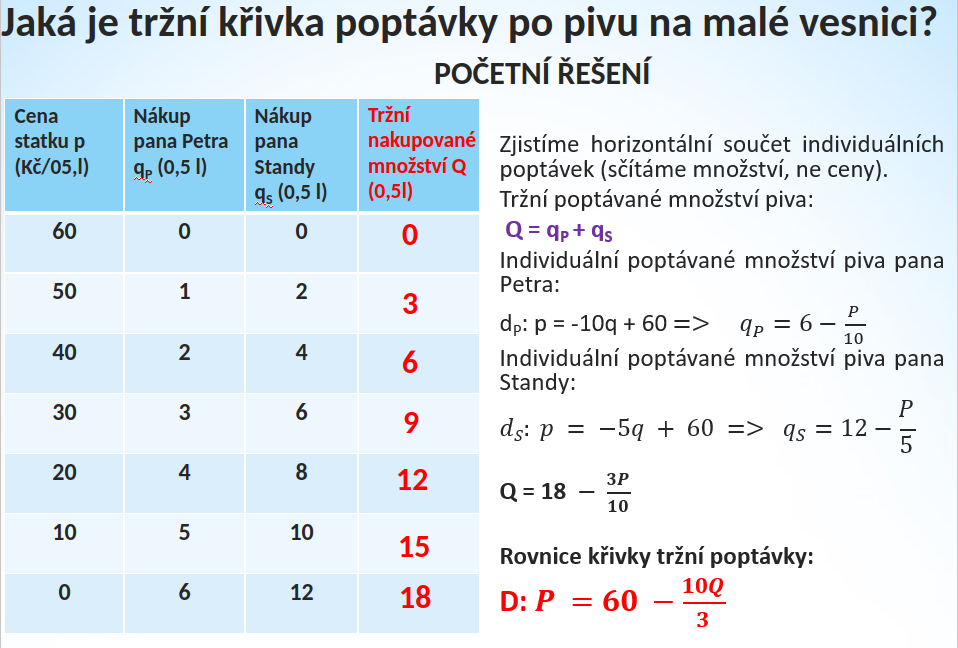
\includegraphics[width=16cm]{images/07_odvozeni_poptavky.png}

\subsection{Faktory ovlivňující poptávku}
\begin{itemize}
    \item Cenové faktory - posun po poptákové křivce
    \begin{itemize}
        \item Změna ceny statku
    \end{itemize}
    \item Necenové faktory - posun poptávkové křivky
    \begin{itemize}
        \item Změna důchodu spotřebitelů
        \item Změna ceny komplementů/substitutů
        \item Móda
        \item Očekávaná změna ceny zboží
    \end{itemize}
\end{itemize}

\subsection{Cenová elasticita poptávky}
\begin{itemize}
    \item $E_{PD}=\frac{\%\Delta Q}{\%\Delta P}$, kde $Q$ je množství a $P$ je cena
    \item Závislost mezi změnou množství a změnou ceny
    \item typy:
    \begin{enumerate}
        \item Dokonale elastická poptávka, $E_{PD}\rightarrow \infty$, poptávané množství nezávislé na ceně
        \item Elastická poptávka, $E_{PD}>1$, jednoprocentní změna ceny vyvolá větší než procentuálně jednotkovou změnu objemu poptávaného zboží (např. pokles ceny statku je doprovázen takovým zvýšením realizovaných prodejů, že se celkové tržby zvýší.
        \item Jednotkově elastická poptávka, $E_{PD}=1$ 
        \item Neelastická poptávka, $E_{PD} < 1$
        \item Dokonale neelastická poptávka, $E_{PD}=0$, poptávané množství se nemění.
    \end{enumerate}
\end{itemize}

\subsection{Důchodová elasticita poptávky}
\begin{itemize}
    \item $E_{ID}=\frac{\% \Delta Q}{\% \Delta I}$, kde $Q$ je množství a $I$ je výše důchodu
    \item citlivost reakce spotřebitele v nakupovaném množství statku na změnu důchodu
    \item typy:
    \begin{enumerate}
        \item Normální statek, $E_{ID}>0$
        \item Luxusní statek, $E_{ID}>1$, spotřeba roste rychleji než důchod
        \item Nezbytný normální statek, $0<E_{ID}<1$, spotřeba roste pomaleji než důchod, ale roste
        \item Podřadný statek, $E_{ID}<0$, spotřeba klesá se zvýšením důchodu
    \end{enumerate}
\end{itemize}

\subsection{Křížová elasticita}
\begin{itemize}
    \item $E_{CD}=\frac{\% \Delta Q_1}{\% \Delta P_2}$, kde $Q_1$ je množství jednoho statku a $P_2$ je cena druhého
    \item Závislost mezi změnou ceny jednoho statku a změnou poptávaného množství druhého
    \item typy:
    \begin{enumerate}
        \item Substituty, $E_{CD}>0$, cena jednoho se zvýší, koupíme radši jiný, zástupný statek
        \item Komplementy, $E_{CD}<0$, cena jednoho se zvýší, tak nechceme kupovat ani druhý,
        který se používá s prvním (např. zdrahne elektronika, bude se prodávat méně beden na PC)
    \end{enumerate}
\end{itemize}
